\documentclass{article}
\usepackage[utf8]{inputenc}
\usepackage{url}
\usepackage{graphicx}
\usepackage{hyperref}

\begin{document}
\title{Facial Recognition Project}
\begin{figure}
    \centering
    
\includegraphics[scale = 0.25]{gmit}
    \label{fig:gmit}
\end{figure}
\author{Arnas Steponavicius
        \and Aaron Moran
        \and Thomas Kenny}
\maketitle
\underline{Project Repository: \url{https://github.com/Moran98/facial-recognition}}
\tableofcontents
\newpage
\section{Introduction}
When we formed our team there was many ideas floating around of what to design and make. We tried to think of an idea that was new and exciting for the three of us. We wanted to make design and make something that was challenging and would improve our ability as software students. The idea we settled on was Facial Recognition. 
    
With extensive research into this field we looked at many languages to use. We thought it would be a good idea to learn a new language while working on this project. This language was Python. 
Python is one of the top languages used worldwide at the moment so we thought this would be beneficial for us to learn this language. We chose this language for various reasons, one of these reasons being that there is various packages python offers. We found online that there is a library called \textbf{face\_recognition} that suited our needs for this project. 

We had various meetings in the beginning to find the pros and cons of Facial Recognition. We had to map out the project and treat this like it was a job. This included making a plan of what we wanted to have done to present in our weekly meetings, breaking up the project into steps so we wouldn't’t get overwhelmed or held up on one task and discussing what each member of the team would focus on. Each task will be explained in further detail.

GitHub was vital with our project. It was important that we constantly used GitHub to display the progress we were making. We could handle issues we were having, test different ideas and we could all be on the same page as we work. We mainly tracked our developments and any bugs which had to be fixed by using the Issues section on GitHub, Once the issue was resolved we would mark is as complete. This made each member of the group aware of a bug and then we could all attempt to resolve the issue.

\maketitle
\section{System Requirements}
\textbullet{ Python 3.3+ } \newline
\textbullet{ C/C++ compiler installed }\newline
\textbullet{ CMake \url{https://cmake.org/download/ }}\newline
\textbullet{ Camera}

\maketitle
\section{Technology Used}
\textbf{\underline{Language: }}\newline
\newline
\textbullet{ Python}\newline
\newline
\textbf{\underline{Framework: }}\newline
\newline
\textbullet{ Django }\newline
\newline
\textbf{\underline{Dependencies: }}\newline
\newline
\textbullet{ pip install face\_recognition }\newline
\textbullet{ pip install opencv-python }\newline
\textbullet{ pip install numpy }\newline
\textbullet{ pip install pillow }\newline
\newline
\newline
\newline
\newline
\newline

\maketitle
\section{Architecture of the solution }
We designed this project to be user friendly and simplistic. From the following images you can see the UI is simple which makes for a better user experience.
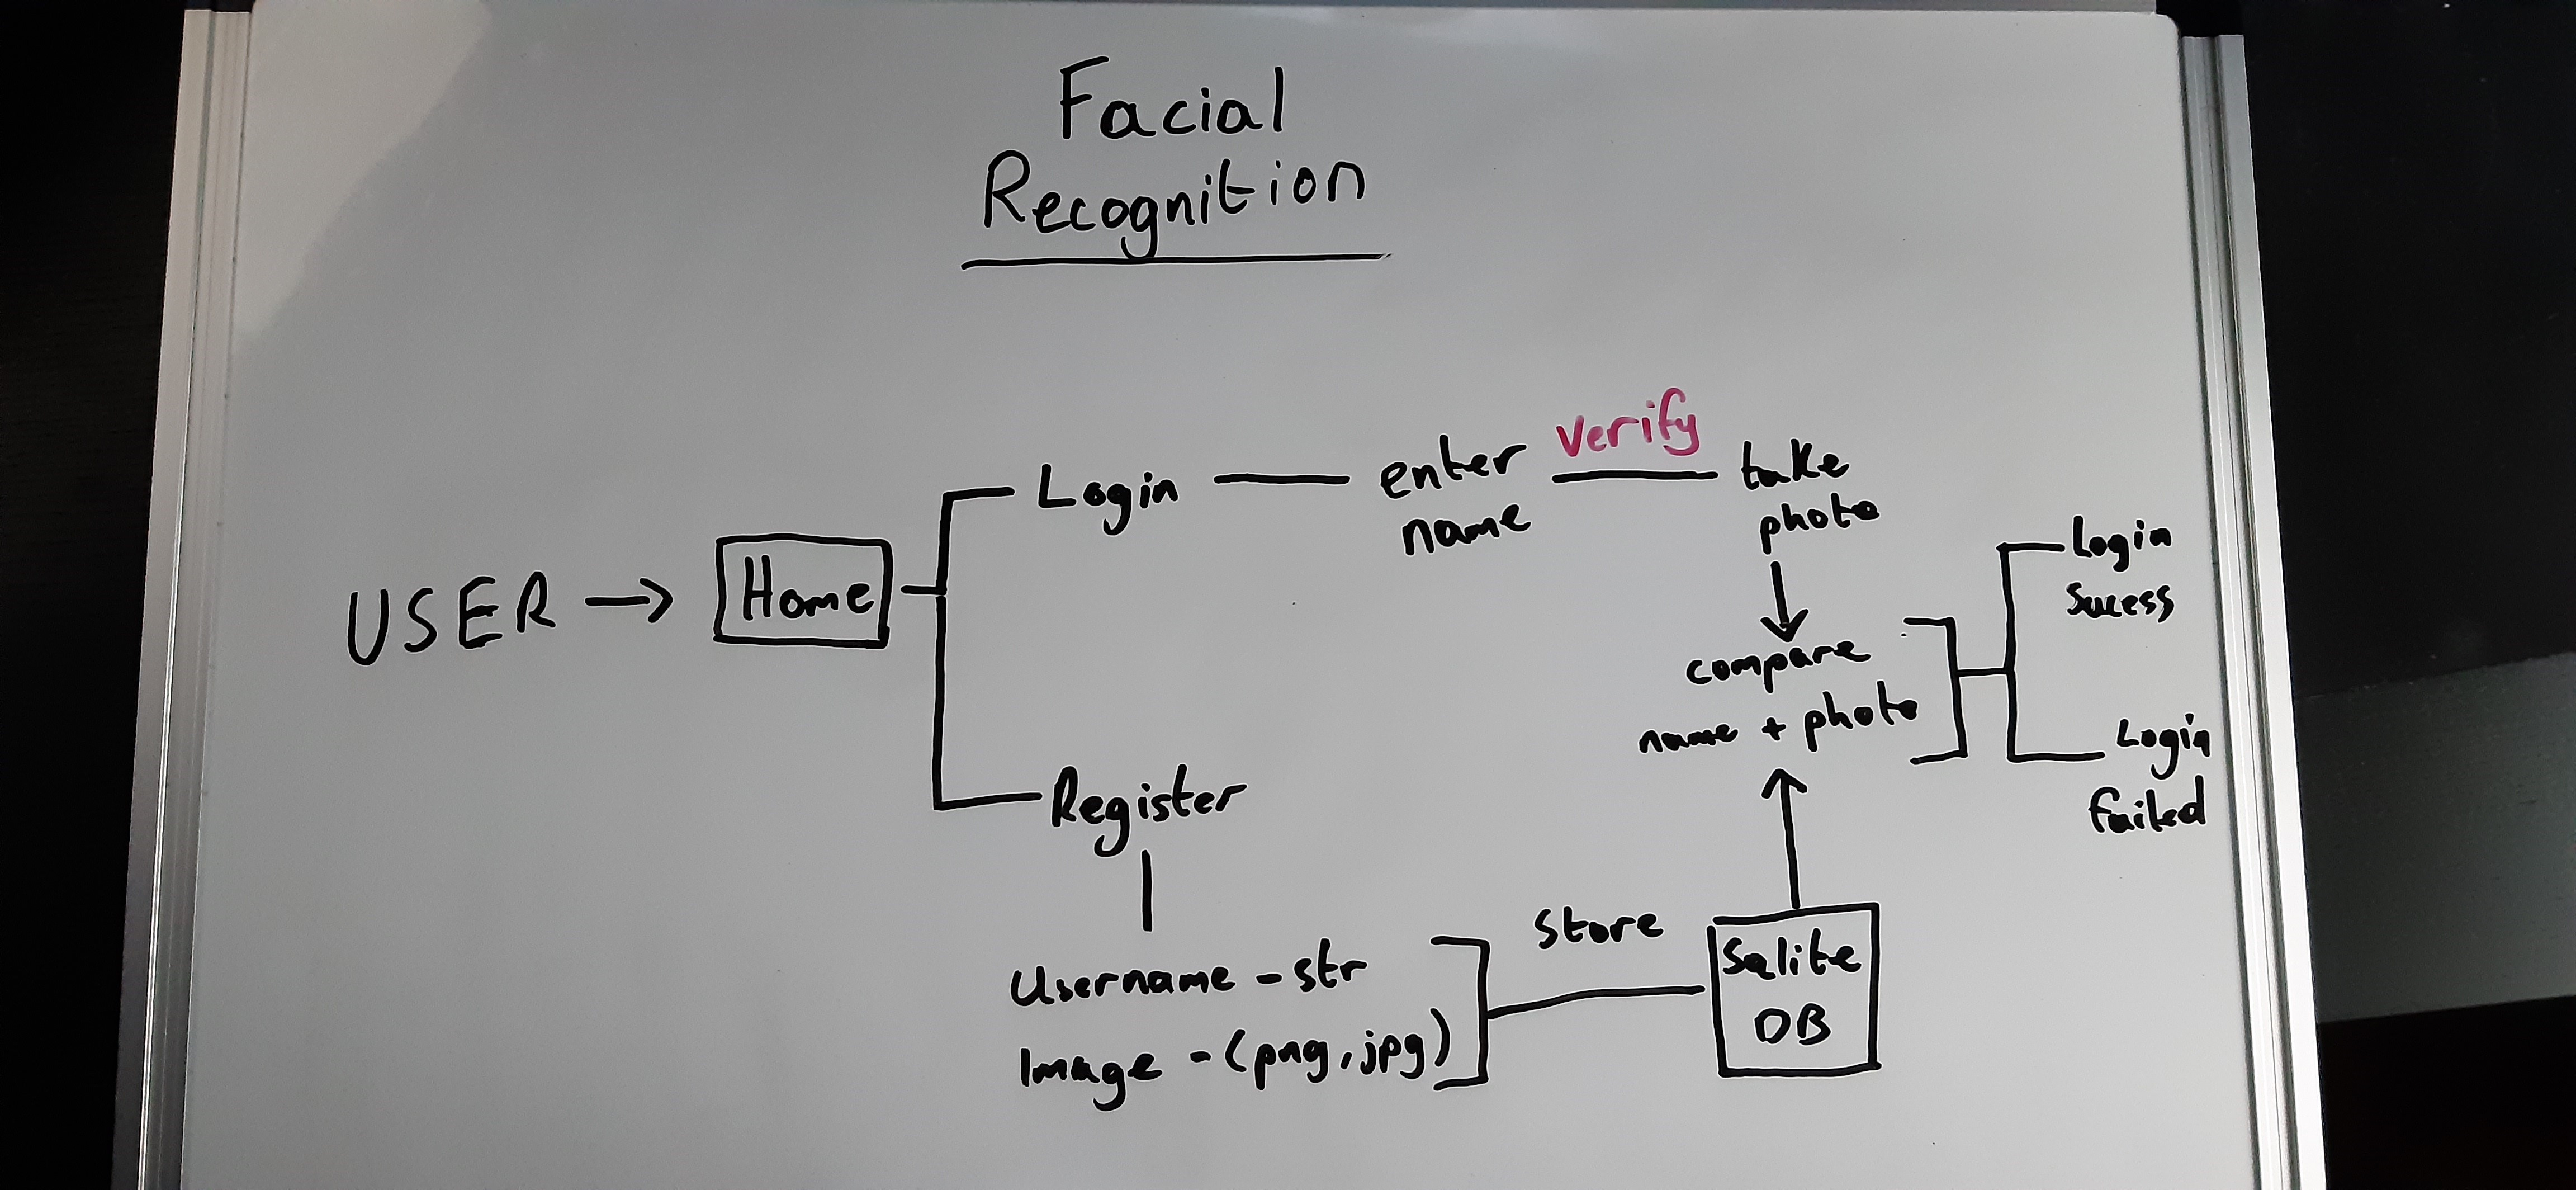
\includegraphics[scale = 0.1]{document/diagram1.jpg}
The thought we had in mind for this project was for companies to use our Register and Login software and enhance it to suit their needs.This software can be easily tailored from colour to design with customer request.
The UI design is located on one CSS file. This makes for updating style simple and quick to achieve.
The python and HTML files are formatted for ease of navigation. The order of the files are simple and understandable. This makes for an easier approach to edit specific files. We made sure to have good package management so any new adaptations to the project were easy to navigate to this reduced any clutter files which were not of any use to the project.

\begin{flushleft}
\section{Design Methodology}
When we were deciding on how our User Interface should be implemented we drew out a few designs using wire frame. After creating multiple styles and designs, we all agreed on the most simplistic design that does not overwhelm the user with information and was very easy to use. As you can see the design is very simple and clear. We thought about adding more to the pages like a template website but decided on "a less is more" approach to the design. Each page implements a layout.html file that stores all the style sheet's that have been used and bootstrapping for each of the web pages. Django has an organized folder system to make the project cleaner and allows easy linking between style sheet's and HTML files. The design is user friendly and self explanatory for the user in terms of instructions and usability. 
\newline
\newline
\newline
\newline


\begin{flushleft}
\textbf{\underline{Home Screen:}}
\end{flushleft}

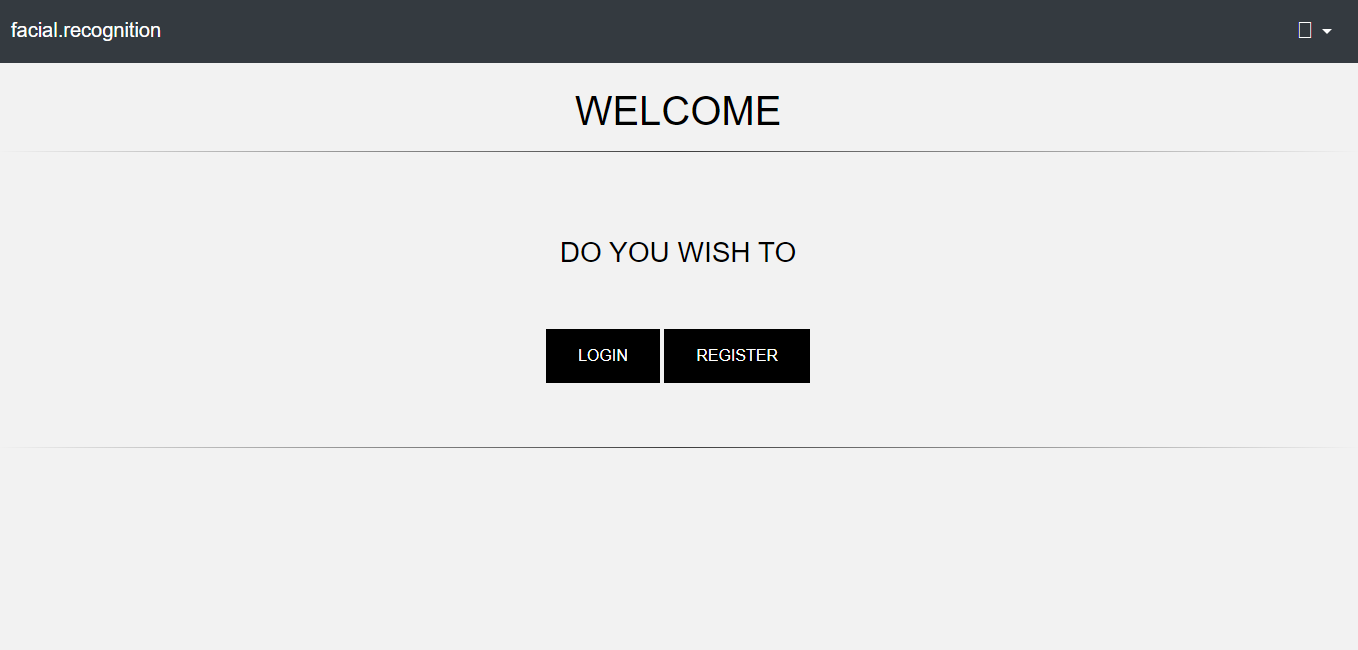
\includegraphics[scale = 0.25]{document/WelcomeScreen.PNG}

\begin{flushleft}
\textbf{\underline{Login Screen:}}
\end{flushleft}

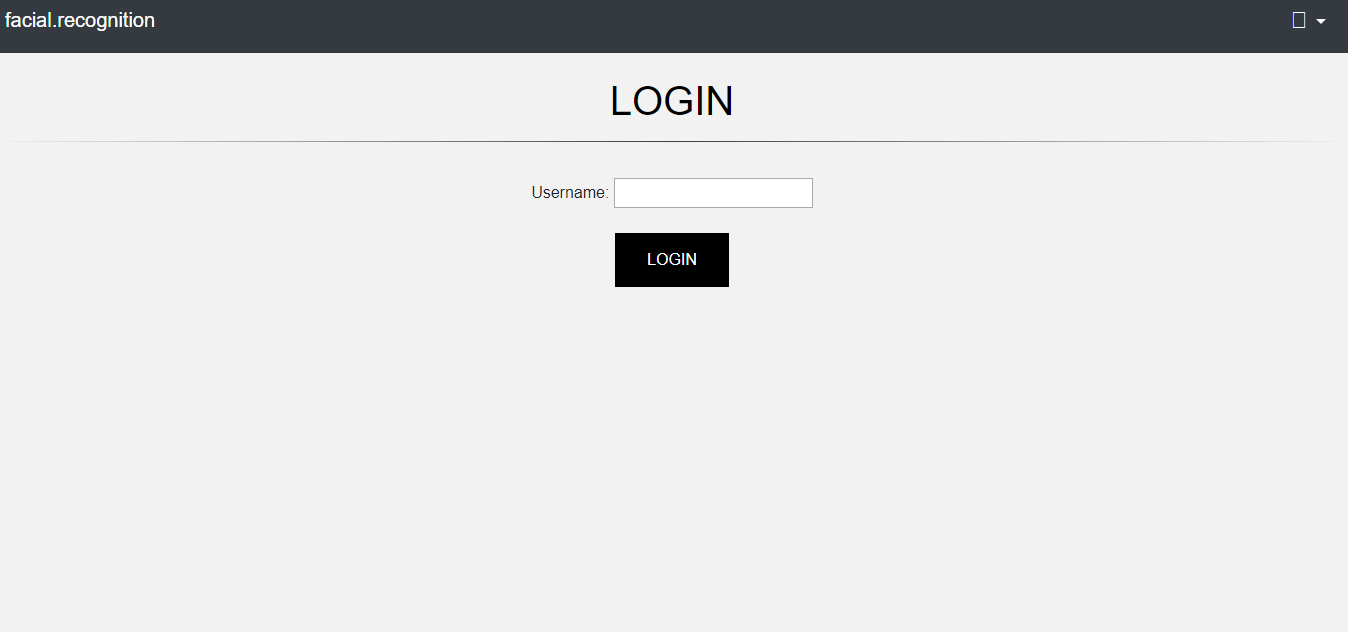
\includegraphics[scale = 0.25]{document/Login.PNG}
\newline
\newpage
\begin{flushleft}
\textbf{\underline{Register Screen:}}
\end{flushleft}

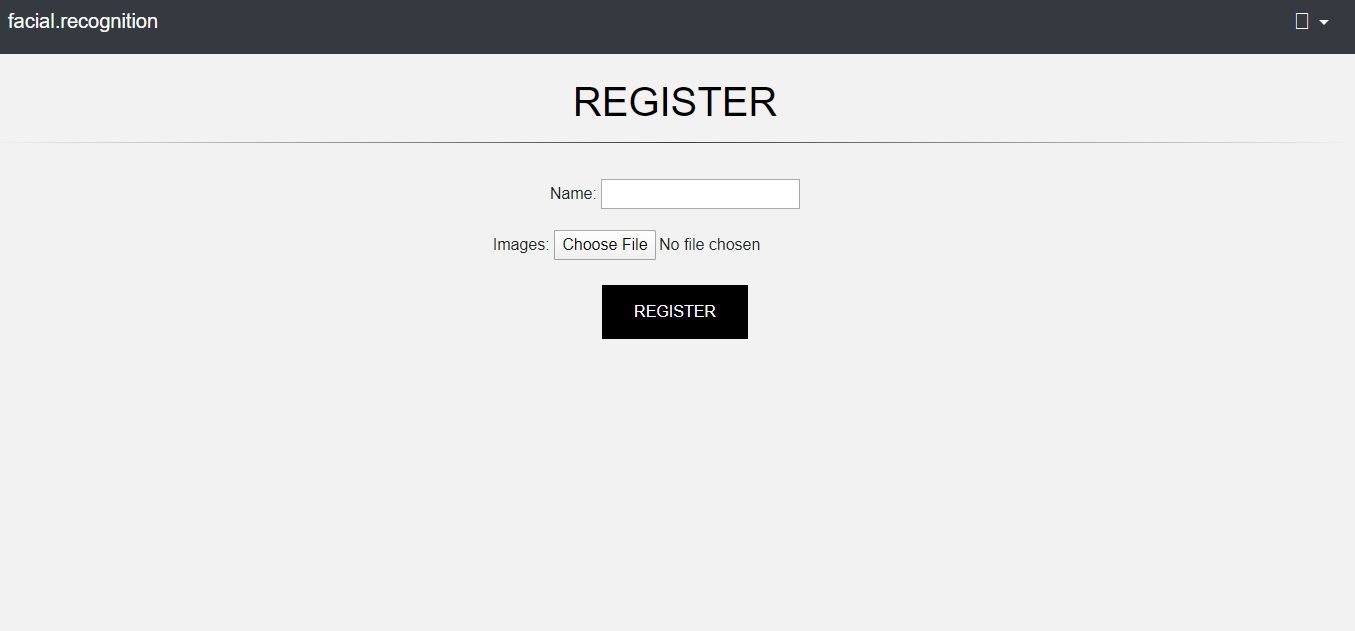
\includegraphics[scale = 0.25]{document/Register.PNG}
\label{fig:WebsiteImages}
\newline
\newline
\newline

\begin{flushleft}
\section{Features}
The main aim of the features implemented in this project is to provide security by using facial recognition to be able to access the inner system. Whether this software will be used for a personal use or within a company environment.
\newline

\textbullet{ When the user runs the program they will be greeted with the option of Login or Register. The home page is very simple, user friendly and self explanatory. }

\textbullet{ The second feature is the register page which needs the user needs to submit their name and a clear frontal picture of themselves. These details are then saved to the database. The user must enter in details into the required input boxes or they cannot proceed in creating an account. Both options are required so no user is signing up without a registration photo.}

\textbullet{ The main feature is the login. The user needs to enter a valid name that has been registered otherwise an error will pop up. If the name is valid the user is then brought to the verification page, where they need to take a photo of themselves. If the photo matches the image the users registered image they are let through into the site.}

\textbullet{ Administrator access is a feature Django provides the developers with and is a very useful feature that can be used to create, update or delete a user profile within the database. This feature made it simple for each one of us to test our project and to visually see if the correct details were being stored for the user in the database.}

\newpage

\section{Limitations and Bugs}
As with any programming project we encountered a plethora of bugs and limitations whilst working on this project. The most frustrating one of all was in the initial stages of the project. We had chosen to work with the \textbf{Flask} framework and had a problem with taking an image on the web page using JavaScript, encoding the image and sending it to our database via Ajax. This problem that we had set us back for a while until we ultimately decided to swap framework to \textbf{Django}. 

When we began our project with Flask we faced issues such as installations for different python packages working on specific operating systems smoothly and then not working as expected on other operating systems. We also faced problems witch collaboration on the project as a new push to the repository would affect another contributors ability to develop the program as installations were not installing correctly. Thanks to Django we were able to just install the Django package and then work on developments without any issues.

Within a few days of making the switch we managed to get our images uploading to a database and then setting up the routes for the other links in our web application.

Another bug we had encountered was an Index out range error whenever an image that did not have a recognisable face on it was loaded in, but it was tackled with simple try catch statement.

For further insight into issues we faced you can view them in our GitHub repository Issues section where we often assigned issues our project was facing and solved them as a group together. This helped us to learn problem solving as a team as well as individuals.

\section{Testing Plans}
We went through extensive testing whilst making this project. Every commit that was uploaded to our repository was tested beforehand before the commit.
Testing played a vital role in the production of our project. We had to make sure each small part was tested so the user experience would be up to standard. We found problems along the way whilst making of the project. One of these problems we encountered was the upload of an image.

Through White Box Testing we discovered and fixed the errors we had. We also use a Black Box Testing approach to see what the user experience was like on a user that wasn't apart of the production group. This gave us insight into how a user without experience of using the website was able to navigate throughout the project without any issues and what we need to improve on. 

We tested the the features of our project a countless amount of times and noticed a few bugs in the process of this, whenever we found a new bug in the system we worked on a fix and almost always faced another issue somewhere else but we worked as a group to overcome these issues. Testing was such a vital part of our project since our project is based around a user login and register system it would be a major flaw to allow an user into the incorrect account. This way we made sure there would be no faults or bugs remaining when registering and logging in once the project was completed.

\section{Recommendation for Future Development}
For future development we will take on board everything we learned whilst doing this project. The team enjoyed the challenge of working with and learning a new language. This is something we can carry over to future development.

We now know even with extensive testing you can still hit many roadblocks along the way. Our experience of this was the framework. At the start we decided on using flask as our framework but we encountered multiple problems with our database and images. With this in mind we made the choice to switch to \textbf{Django}. This decision was made for the better of the project and once changed the project came together quickly. These types of problems will be beneficial for us in the future. Our learning of GitHub will be useful in the future. Through various lectures we learned how to use Issues on GitHub this made dealing with problems more manageable.

For future development the approach we would definitely take and begin with would be to fully research and decide on our design decisions, frameworks, implementations, time-management and methodologies. This way we can have it fully scaled out what we are going to achieve week by week. By implementing more structure we may not face any issues like changing frameworks or being indecisive on a design decision. This way we can get our project completed in a timely manner before our deadlines and then have extra time to clean up the code and increase our testing of the project. 


\section{Conclusions}
To conclude, \newline
The making of this project proved to be no easy task.Through making this project each of us learnt and improved various skills, whether it be improved communication skills, working as a team, time management, design and coding ability.

This project will benefit us in our future careers as Software Developers as we moved out of our comfort zones and learned a new programming language and designed and completed a project within a given time frame. After finishing the project and looking back we feel we could have done better in some areas. For example we could have researched more into certain areas such as adding specific user detail's to the database, selecting a framework which systems suited us most and also keeping consistent with developments within the project, This however gave us challenges to overcome.

We now know how to deal with these types of problems if they were to occur in the future when we are working professionally as Software Developers. Ultimately, we are pleased with the project we have produced and enjoyed the independent learning process of a project assigned with free roam of ideas to implement.

\section{Acknowledgements}

\underline{\url{https://www.fullstackpython.com/table-of-contents.html}}
\newline
\underline{\url{https://www.fullstackpython.com/django.html}}
\newline
\underline{\url{https://www.fullstackpython.com/flask.html}}
\newline
\underline{\url{https://www.sqlalchemy.org/}}
\newline
\underline{\url{https://www.pythonpool.com/face-detection-using-opencv-and-python/}}
\newline
\newline
\textbf{face\_recognition library}
\underline{\url{https://github.com/ageitgey/face\_recognition/issues/175}}
\newline

\textbf{Django Cheat Sheet:}
\underline{\url{https://github.com/lucrae/django-cheat-sheet/}}
\newline
\newline
\textbf{Django File Uploading:}
\underline{\url{https://docs.djangoproject.com/en/3.0/topics/http/file-uploads/}}
\newline

\underline{\url{https://medium.com/@muehler.v/node-js-opencv-for-face-recognition-37fa7cb860e8}}
\newline

\textbf{Directory Traversal in Python}
\underline{\url{https://www.pythoncentral.io/how-to-traverse-a-directory-tree-in-python-guide-to-os-walk/}}
\newline
\newline
\textbf{Sentdex}
\newline
\underline{\url{https://www.youtube.com/channel/UCfzlCWGWYyIQ0aLC5w48gBQ}}
\end{flushleft}
\end{flushleft}
\end{document}
